\documentclass[19pt]{beamer}
\usepackage{graphicx}

% \title{Stereo Vision}
% \author{Robert Washbourne}
% \date{\today}

\begin{document}

% \maketitle

\begin{frame}
\frametitle{Introduction}

Imagine driving in the dark, alert but not noticing a deer cross the road. Using stereo matching methods to see what is close, your car could detect the deer and brake before you even saw the obstacle. The cameras would find distances, and sensing something closer than 20 feet, send the location of the deer to the computer. The computer would see that driving over this would be catastrophic for the car, and turn on the brakes. The deer, and you, would be safe.
\end{frame}


\begin{frame}
\frametitle{What is stereo matching?}

Stereo matching is a topic in computer vision where two images, taken from aligned cameras several centimetres apart, are processed and depth data is returned. For example, taking two images and using a simple algorithm, a grayscale image is returned, with lighter pixels closer than darker pixels. Here is an example, generated with my code.\\[20pt]

\centering
\setlength\tabcolsep{0.005\textwidth}
\begin{tabular}{ccc}
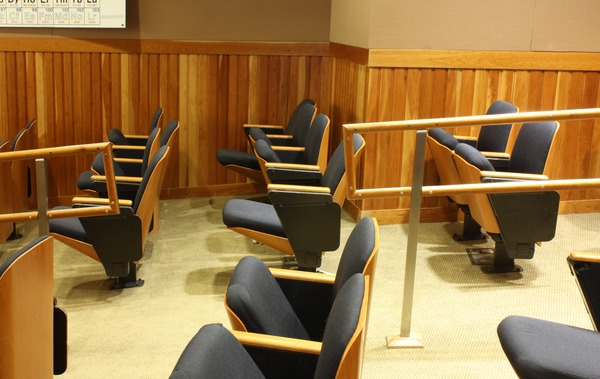
\includegraphics[width=0.31\textwidth]{images/im0-600.jpg} &
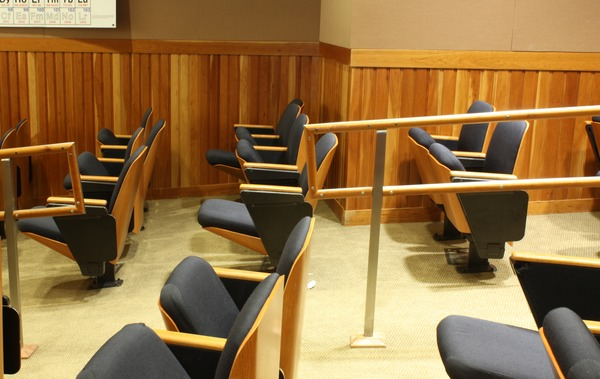
\includegraphics[width=0.31\textwidth]{images/im1-600.jpg} &
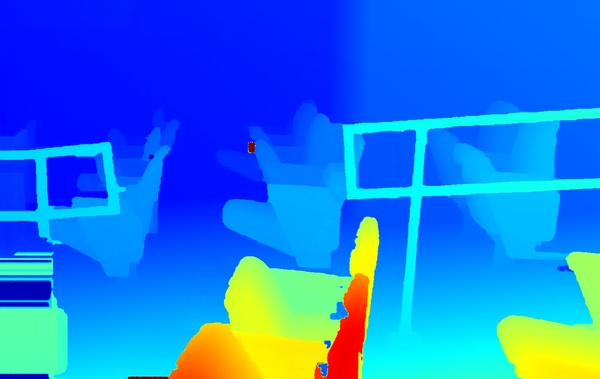
\includegraphics[width=0.31\textwidth]{images/disp-600.jpg} \\[2pt]
Left image & Right Image & Stereo matching result \\
\end{tabular}

\end{frame}


\begin{frame}
\frametitle{Workflow}
\begin{enumerate}
    \item Calibrate stereo webcams
    \item Capture images from stereo webcams
    \item Split images into one pixel high rows and correlate
    \item Estimate pixel distance
    \item Apply edge preserving median filter
    \item Return the final disparity map 
\end{enumerate}
\end{frame}

\begin{frame}
\frametitle{Workflow 1: Calibrate stereo webcams}
\end{frame}

\begin{frame}
\frametitle{Workflow 1: Capture images from stereo webcams}
\end{frame}

\begin{frame}
\frametitle{Workflow 1: Split images into 1 pixel high rows and correlate}
\end{frame}

\begin{frame}
\frametitle{Workflow 1: Estimate pixel distance}
\end{frame}

\begin{frame}
\frametitle{Workflow 1: Apply edge preserving median filter}
\end{frame}

\begin{frame}
\frametitle{Workflow 1: Return the final disparity map}
\end{frame}


\end{document}